
%*****************************************
\chapter{Case Study}\label{ch:fifth}
%*****************************************

In the following chapter, we will present the user case study which we conducted, to validate the findings of Anonymous et al. \cite{anonymous}, presented in Chapter \ref{ch:third}. Our goal was to verify that \textit{orientation} time truly has an influence on the perceived efficiency of an authentication mechanism, and that users prefer concepts that have short \\textit{orientation} rather than long \textit{orientation}. We will commence by presenting the design of our study. We will then proceed by explaining how we recruited our participants and also present their demographic. Next, we will provide a walkthrough of the study's procedure and move on the illustrating our quantitative and qualitative results.  

\section{Design} \label{5.1}

The user case study was designed as a field study and was conducted on campus of the computer science department of Uni Bonn and at the author's home. The tool used for the study was the application \underline{\textbf{FiPa}} which we presented in Chatper \ref{ch:forth}. Our independent variable was \textit{ratio} and it had three levels:
\begin{enumerate}
    \item \textcolor{blue}{Long} orientation - \textcolor{red}{Short} input (abbrv. \textit{Long/Short}), 
    \item \textcolor{red}{Short} orientation - \textcolor{blue}{Long} input (abbrv. \textit{Short/Long}), 
    \item \textcolor{red}{Short} orientation - \textcolor{red}{Short} input (abbrv. \textit{Short/Short}). 
\end{enumerate}

The order of the ratios was counterbalanced amongst the participants (see figure \ref{fig:permutation}. Data was collected quantitatively by measuring the \textit{orientation} and \textit{input} time for each of the ratios. We also documented the number of errors made during \textit{orientation} and also when a false input was made. This information was automatically documented and stored in a local database during the interaction. Data was also collected qualitatively through a questionnaire, which required study participants to evaluate the aesthetic of our application, the ratios ( 1. and 2. ), and to also choose which of the two ratios they preferred most. The study was intentionally designed to be as short and simple as possible, such that we could receive the information we needed from our participants without requiring too much effort or concentration. On average, the duration of our study was 20 minutes per participant. 

\section{Participants} \label{5.2}

We were able to recruit 25 participants for our study. Initially, students were informed about the study through a social platform for the computer science students of Uni Bonn. Another part was collected on campus of the university's computer science department, and four participants were acquaintances of the author. There was no premise for participating in the study, meaning anyone was eligible to partake. After extracting the participants that made search and input errors out of our sample, we remained with 19 valid data entities, of which 13 (62.4\%) were male and 6 (31.6\%) were female. The average age was 21 years, with 17 being the youngest and 31 being the oldest. The majority of the participants (78.9\%) had an IT-Background and were computer science students. Also, all of the participants, except for one, used a screen lock for their smartphones, of which 42.1\% used \textit{Pin}, 36.8\% used \textit{Pattern}, and 15.8\% used \textit{Password} (see figure \ref{fig:demo}).  

\begin{figure}[t!]
\centering
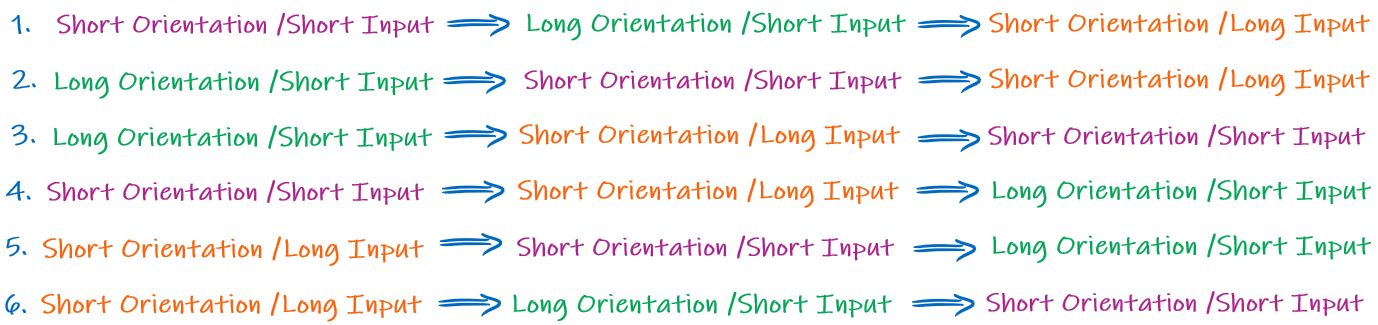
\includegraphics[width=14cm, height=4cm]{Chapters/graphics/permutation.PNG}
\caption{The order in which the three ratios were permuted in the application, throughout the study.}
\label{fig:permutation}
\end{figure}


\section{Procedure} \label{5.3}
The study was held for each participant, separately. We began by roughly explaining the purpose of our study:

\begin{center}
\textit{To analyse certain factors in smartphone authentication that might play a role in its perceived efficiency.}    
\end{center}

We also emphasized our main focus was the improvement of usability in authentication mechanisms and that the security aspect was outside the scope of our research. Also, we clarified that testing \underline{\textbf{FiPa}} was not intended to evaluate their cognitive skills or intelligence. We wanted our participants to feel as comfortable as possible during the course of our study and that they did not feel nervous or put under pressure in any way. This was important to us because we wanted their performance and our collected data to be as close to the results of a real-life scenario as possible. \\

Next, we described the structure of our application, \underline{\textbf{FiPa}}. We explained that it was an interaction system which emulated an activity, similar to an authentication concept. Furthermore, we mentioned that the application presented a series of small "challenges", for them to solve. With "challenges" we meant the \textbf{mental} and \textbf{practical} tasks, explained in Chapter \ref{ch:forth}. These simple challenges were demonstrated with the help of a simple paper prototype.\\

\begin{figure}[t!]
\centering
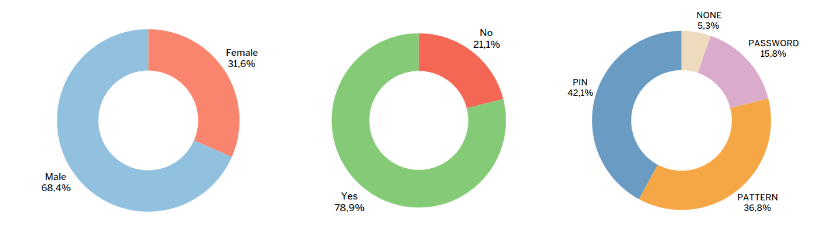
\includegraphics[width=15cm, height=5cm]{Chapters/graphics/Demos.PNG}
\caption{Demographic data on the gender (left), IT-Background (middle) ration and on the personal screen lock choice (right) of our participants.}
\label{fig:demo}
\end{figure}

After ensuring that our participant had no further questions, it was time for them to test \underline{\textbf{FiPa}}. First, they were asked to begin with the training-segment of the application [SECTION !!!!]. The purpose of the training-segment was to ensure that our participant understood the concept of \underline{\textbf{FiPa}}, to prevent that our measured times being influenced by a lack of understanding of what to do. The participant could repeat the training-segment as often as they wanted, until they felt ready to start the actual testing of the application. We guided them through the training-segment, when help was needed, and took the chance to explain to them the certain features and aspects of the application. \\

When the participant felt ready to start the test, we first entered a user-id, to be able to pair their measured data with their qualitative data, in the result-evaluation. We did not intervene, while they were working on the test. Once they were done, they were given a questionnaire to fill out. In the end, each participant was compensated with 5 Euros.



\section{Results} \label{5.4}

Throughout this section we will define a \textit{ratio} as a \textit{combination}. We used this terminology during our study to simplify the notion of the word \textit{ratio} to our participants, as a \textit{combination} of different phase lengths.

\begin{figure}[t!]
\centering
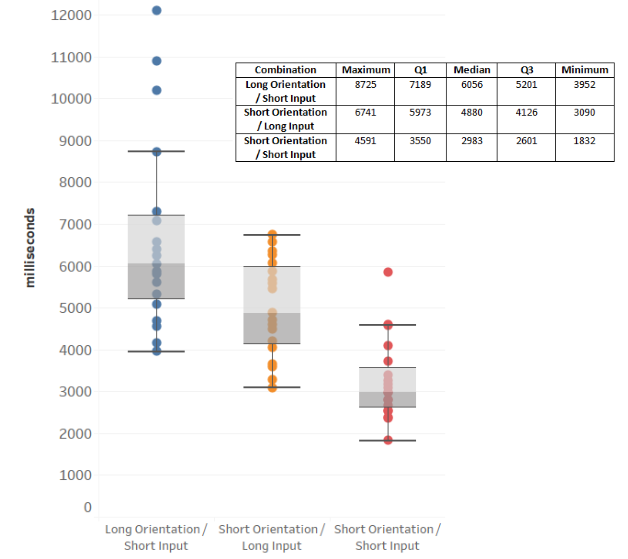
\includegraphics[width=13cm, height=11cm]{Chapters/graphics/Combinations.png}
\caption{A boxplot of the overall times of each combination/ratio.}
\label{fig:combination}
\end{figure}

\subsection{Measurements}

 As mentioned in Section \ref{5.4}, \textit{orientation} and \textit{input} times were measured for each of the \textit{combinations}, realized in the application. As we know, each \textit{combination} presents three different challenges (couples, see Section \ref{4.2.2.4}). Analogous to our measurement approach in section \ref{4.2.2.4}, we considered the first and second challenge of each combination to be an exercise for the user. Despite the training-segment, participants made a significant amount of mistakes in the first two challenges, and made very little to non in the third. To provide ourselves a clean collection of data sets, we excluded all of the data entities which included any search fails or unsuccessful input activities. This gave us a clean collection of 19 data sets. \\

We will start by analysing the measured times of each combination (see figure \ref{fig:combination}). Although, we designed the combinations \textit{Short/Long} and \textit{Long/Short} (see Section \ref{5.1}) to be as close to each other as possible, in terms of their duration, our results show that they had a temporal difference of 1176 ms, on average\footnote{We will present an assumption for why that is, later in our discussion (see Chapter \ref{ch:sixth}).}. The combination \textit{Long/Short} had the longest duration, followed by \textit{Short/Long} and, lastly, \textit{Short/Short}.  Interestingly, we noticed that the average time of all three average periods combined (4639 ms), differs slightly from the average duration of the \textit{combination} \textit{Short/Long}. 

We took it upon ourselves to thoroughly examine the times of each single phase of the combinations and compare them to each other, to see how the crossing phases (short or long) differ from each other (see figure \ref{fig:times}). We did not notice a significant difference between the short \textit{input} times of combination \textit{Short/Short} and \textit{Long/Short}. Nonetheless, it is interesting to see that, on average, participants needed slightly less time to enter the pattern in \textit{Long/Short} than they needed in \textit{Short/Short}, being that patterns in both combinations are the same. \textit{Short/Short} and \textit{Short/Long} show a more notable difference in terms of their average \textit{orientation} times (663 ms). 

\begin{figure}[t!]
\centering
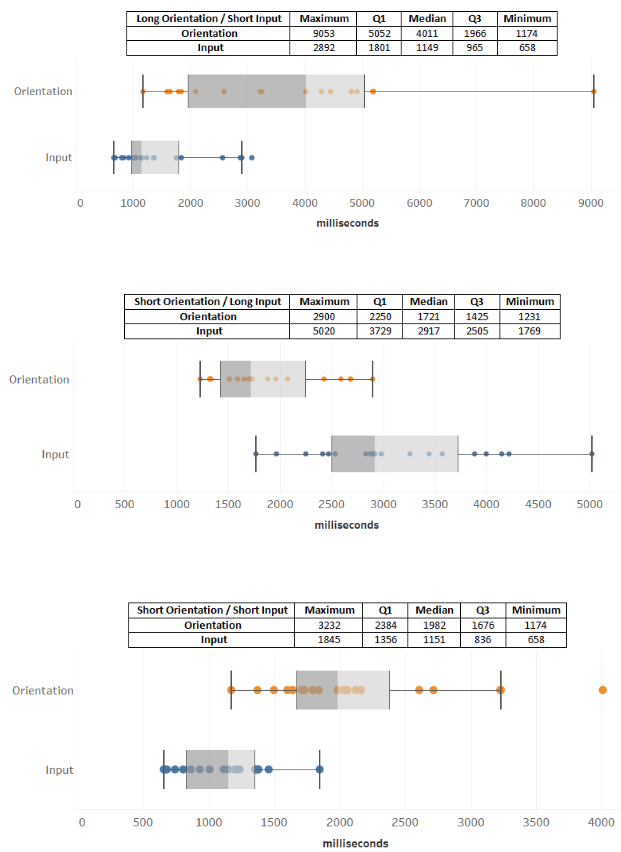
\includegraphics[width=14cm, height=20cm]{Chapters/graphics/Times.png}
\caption{A boxplots of each combination.In each combination we distinguish between \textit{orientation} and \textit{input} times. Top: \textit{Long/Short}; Middle: \textit{Short/Long}; Bottom: \textit{Short/Short}.}
\label{fig:times}
\end{figure}

\subsection{Users' Perception}

We decided to focus the qualitative evaluation on the \textit{combinations} on \textit{Long/Short} and \textit{Short/Long}. We assumed that by setting them against each other, we could get precise insight on which one the participants favor more. To ensure that they did not confuse the \textit{combinations} we gave them a illustration of the two \textit{combinations} and verbally explained it to them.

The participants were asked to evaluate both \textit{combinations} separately, through a five-point Likert scales. When asked whether they found the searching process (\textbf{mental task}) of \textit{Long/Short} annoying, the average answer was \textit{neutral}. Also, most participants were able to memorize (89\%) and enter (84\%) the pattern (\textbf{practical task}) easily (see figure \ref{fig:likert}). In contrast, 79\% \textit{strongly disagreed} and 21\% \textit{disagreed} that the search process of the combination \textit{Short/Long} was annoying. Also, the majority agreed that the pattern was easy to memorize (100\%) and enter (89\%) (see figure \ref{fig:likert}).
 
 \begin{figure}[t!]
\centering
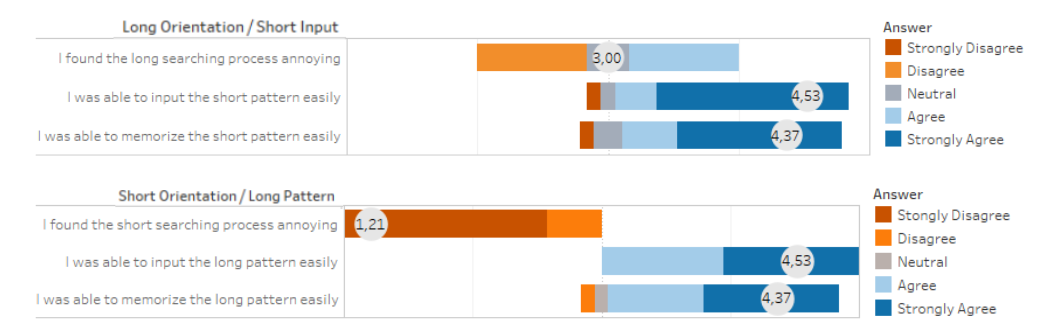
\includegraphics[width=15cm, height=5cm]{Chapters/graphics/Likert1213.PNG}
\caption{An evaluation of combinations \textit{Long/Short} and \textit{Short/Long} using five-point Likert scales. }
\label{fig:likert}
\end{figure}

Next, the participants were asked certain questions, as seen in figure \ref{fig:likert2}, where they had to actively choose which of the both combinations they found applied more. These questions were also answered through Likert scales. When asked which of combination they found required more mental effort, the majority (68\%) chose \textit{Long/Short}, about 16\% chose \textit{Short/Long} and the rest saw no difference between the two. 
About 79\% thought that \textit{Short/Long} was easier, followed by a 16\% rate of the ones that found \textit{Long/Short} easier. We also asked which of the combinations' patterns they perceived took longer to find and and enter. Fifty-eight percent said that \textit{Short/Long's} pattern easier to enter, 26\% chose \textit{Long/Short}, and 16\% saw no difference. All participants found that \textit{Short/Long} was easier to find. Lastly, we asked them which combination they found to be more efficient. Interestingly, no one actively chose \textit{Long/Short}. Seventy-four percent found \textit{Short/Long} more efficient and 26\% saw no difference. \\


Moreover, we wanted to examine how far participants' perception and estimate of the times differed from the actual ones. So, we asked them to choose which one they found took longer overall. We took each participant's answer and compared it to the combination which took longer, in their execution. In total, 58\% (11) misestimated. Thirty-six percent (4) misestimated \textit{Long/Short} to be longer, where \textit{Short/Long} was true. Eighteen percent (2) thought \textit{Short/Long} was longer and 27\% (3) saw no significant difference. \\

\begin{figure}[t!]
\centering
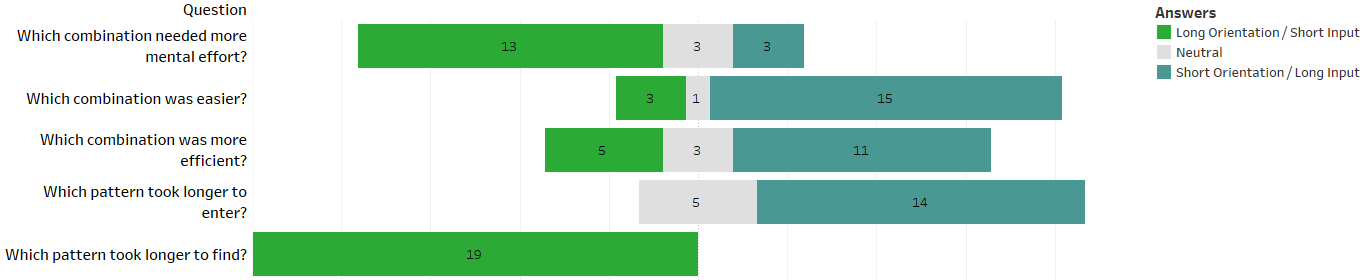
\includegraphics[width=15cm, height=4cm]{Chapters/graphics/Likert2.png}
\caption{Participants were asked to compare the combinations \textit{Long/Short} and \textit{Short/Long} to each other by answering the questions above.  }
\label{fig:likert2}
\end{figure}

To get a clearer understanding of what our participants favored more, participants were asked to say which combination they would choose if they had to use one of them as their screen lock. Participants were also asked to elaborate on their choice, given these four reasons: \textit{It's more efficient / more secure / more difficult / challenging.}\footnote{Multiple answers were possible.}
Forty-two percent (8) chose \textit{Long/Short}, whereas 47\% chose \textit{Short/Long} (see figure \ref{fig:preference}. Most reasons given for \textit{Long/Short} were that is was more secure and more difficult. Only one participant gave the reason \textit{more efficient} and two gave the reason \textit{challenging}. In contrast, most popular reasons for \textit{Short/Long} were \textit{more secure} and \textit{more efficient}. The reasons \textit{more difficult} and \textit{challenging} were only given once, each. One participant elaborated that they would choose the combination because it es easier, especially for when they are tired. Eleven percent chose neither combination for a screen lock and gave the following reasons (see figure \ref{fig:preference}) : 
\begin{itemize}
    \item \textit{"Short/Long is much easier because it's easier to find. It's also much easier to copy => Insecure! I would prefer a mix [of both]."}
    \item \textit{"It don't mind which one, because their use will get easier over time. It really just depends on one's mood."} 
\end{itemize}

\begin{figure}[t!]
\centering
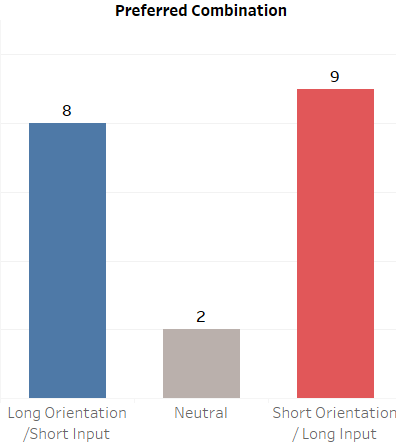
\includegraphics[width=7cm, height=9cm]{Chapters/graphics/preference.png}
\caption{A histogram, representing our participants preferences regarding the combinations.}
\label{fig:preference}
\end{figure}

In addition, we were interested in knowing what impact the built-in error recovery had, on the accomplishment of the tasks. We, therefore, added a question into our questionnaire which only had to be answered if the participant encountered the error recovery phase. The statements were evaluated via a Likert-scale. As a reminder, the error recovery was implemented in the form of a pop-up which appeared during the searching process (mental task). When the user taps on the wrong button for the third time, the pop-up appears, showing a reminder of what the pattern looked like (Section 4.3). Out of 19 participants, only 6 interacted experienced the error recovery (see figure \ref{fig:error}). When asked whether the pop-up helped them find the pattern faster, five of the participants concerned agreed. Only one participant disagreed. Moreover, half of the participants concerned disagreed that the pop-up elongated the searching time, one agreed and two answered with \textit{neutral}. Lastly, when asked whether they found the pop-up annoying, four disagreed, one agreed, and one answered with \textit{neutral} (see figure \ref{fig:error}). \\

ANALYSE THESE PARTICIPANTS !! 


\begin{figure}[t!]
\centering
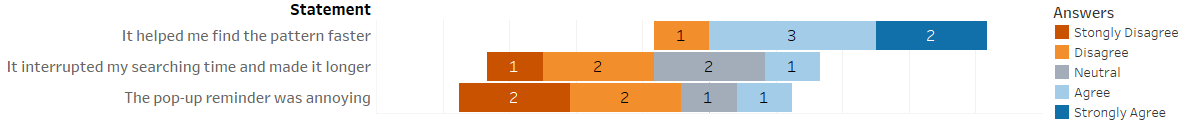
\includegraphics[width=15cm, height=3cm]{Chapters/graphics/ErrorRecovery.png}
\caption{A histogram, representing our participants preferences regarding the combinations.}
\label{fig:error}
\end{figure}





